% % % % % % % % % % % % % % % % % % % % % % % % % % % % % % % % % % % % % % % %
% LaTeX4EI Cheatsheet for Convex Optimization					    Version 1.3
%
% Encode: UTF-8
% % % % % % % % % % % % % % % % % % % % % % % % % % % % % % % % % % % % % % % %


% ======================================================================
% Document Settings
% ======================================================================

% possible options: color/nocolor, english/german, threecolumn
% defaults: color, english
\documentclass[english]{latex4ei/latex4ei_sheet}

\usepackage{bm}
\usepackage{amssymb}
\usepackage{pifont}
\usepackage{amsmath,amsfonts}
\usepackage{calrsfs}
\usepackage{tikz}
\usepackage{caption}
\usepackage{subcaption}
\usepackage{pgfplots}
\usepackage{diagbox}
\usepackage{algorithm}
\usepackage{algpseudocode}
\usepackage{mathtools}\DeclareMathAlphabet{\pazocal}{OMS}{zplm}{m}{n}

\usetikzlibrary{angles, quotes, babel, calc, shapes.misc, bbox}

\tikzset{cross/.style={cross out, draw=black, thick, minimum size=2*(#1-\pgflinewidth), inner sep=0pt, outer sep=0pt},
	%default radius will be 1pt. 
	cross/.default={3pt}}

\DeclareMathOperator*{\argmax}{arg\,max}
\DeclareMathOperator*{\argmin}{arg\,min}

\newcommand{\cmark}{\ding{51}}
\newcommand{\xmark}{\ding{55}}
\newcommand{\notimplies}{%
	\mathrel{{\ooalign{\hidewidth$\not\phantom{=}$\hidewidth\cr$\implies$}}}}

% set document information
\title{LaTeX4EI \\ Convex Optimization}


% ======================================================================
% Begin
% ======================================================================
\begin{document}

\IfFileExists{git.id}{\input{git.id}}{}
\ifdefined\GitRevision\mydate{\GitNiceDate\ (git \GitRevision)}\fi

% Title
% ----------------------------------------------------------------------
\maketitle   % requires ./img/Logo.pdf


% Section
% ----------------------------------------------------------------------
\section{Convex Sets}


\begin{sectionbox}

	\subsection{Combinations}

	\begin{center}
		$\bm{z} = a \bm{x} + b \bm{y} \mid \bm{x}, \bm{y} \in \mathbb{R}^n$
	\end{center}
    
    \begin{tablebox}{@{\hspace{5mm}}c@{\extracolsep\fill}c@{\extracolsep\fill}c@{\hspace{5mm}}}
    	linear 	& $a, b \in \mathbb{R}$ \\
    	conic 	& $a, b \geq 0$ \\
    	affine	& $a+b = 1$ \\
    	convex & $a+b=1, a,b \geq 0$
    	
    \end{tablebox}

	\subsection{Sets}
	
	\begin{tablebox}{@{\hspace{5mm}}c@{\extracolsep\fill}c@{\extracolsep\fill}c@{\extracolsep\fill}c@{\extracolsep\fill}c@{\hspace{5mm}}}
		Set & affine & conic & convex & Examples \\ \cmrule
		Linear Space 	& \cmark & \cmark & \cmark & $\mathbb{R}^n$ \\
		Convex Cone 	& \xmark  & \cmark & \cmark & $\{\bm{p} \mid \bm{p}^\intercal(\bm{x} - \overline{\bm{x}}) \leq 0 \}$ \\
		Affine Set		& \cmark & \xmark & \cmark & $\{\bm{x} \mid \bm{A}\bm{x} = \bm{b}\}$, $\emptyset$, $\{x_0\}$ \\
		Convex Set		& \xmark & \xmark & \cmark & $\{\bm{x} \mid \bm{A}\bm{x} \leq \bm{b}, \bm{b} \neq \bm{0} \}$ \\
		
	\end{tablebox}
	
	\subsection{Cones}
	\vspace{0.3em}
	\textbf{Polar Cone} \\
	\begin{center}
		$\pazocal{X}_p = \{\bm{p} \mid \bm{x}^\intercal\bm{p} \leq 0, \forall \bm{x} \in \pazocal{X}\}$
	\end{center}

	\textbf{Dual Cone} \\
	\begin{center}
		\centering $\pazocal{X}_d = \{\bm{y} \mid \bm{x}^\intercal\bm{y} \geq 0, \forall \bm{x} \in \pazocal{X}\}$
	\end{center}

	\textbf{Conic facts} \\
	\begin{enumerate}
		\item $\pazocal{X}_p$ is a closed convex cone
		\item $\pazocal{X} \subset (\pazocal{X}_p)_p$
		\item If $\pazocal{X}$ closed and convex: $(\pazocal{X}_d)_d = (\pazocal{X}_p)_p = \pazocal{X}$
		\item Cones can be nonconvex
	\end{enumerate}

	\textbf{Geometric interpretation} \\
	\\
	\begin{tabular}{c@{\hspace{1mm}}@{\extracolsep\fill}c@{\hspace{1mm}}@{\extracolsep\fill}c}
		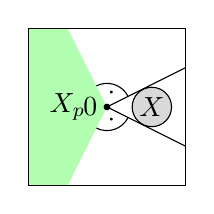
\begin{tikzpicture}[node distance=1cm]
			\coordinate (O) at (0, 0);
			\coordinate (bottomleft) at (-1, -1);
			\coordinate (topright) at (1, 1);
			\coordinate (upper) at (1, 0.5);
			\coordinate (lower) at (1, -0.5);
			
			\coordinate (polarupper) at (-0.5, 1);
			\coordinate (polarlower) at (-0.5, -1);
			
			\fill[fill=green!30] (O)--(polarupper)--(-1, 1)--(bottomleft)--(polarlower);
			
			
			\draw[] (bottomleft) rectangle (topright);
			
			\draw[fill=gray!30] (0.57, 0) circle (0.25cm);
			\node[] (setlabel) at (0.57, 0) {$\pazocal{X}$};
			
			\draw[-] (O) -- (upper);
			\draw[-] (O) -- (lower);
			
			\draw pic [draw, angle radius=3mm, "$\cdot$"] {angle =upper--O--polarupper};
			\draw pic [draw, angle radius=3mm, "$\cdot$"] {angle =polarlower--O--lower};
			
			\draw[fill=black] (0, 0) circle (1pt);
			\node[left] (Olabel) at (O) {$0$};
			
			\node[] (Clabel) at (-0.5, 0) {$\pazocal{X}_p$};
			
			
		\end{tikzpicture} &
		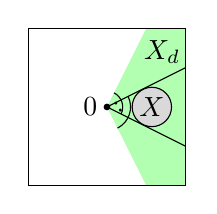
\begin{tikzpicture}[node distance=1cm]
			\coordinate (O) at (0, 0);
			\coordinate (bottomleft) at (-1, -1);
			\coordinate (topright) at (1, 1);
			\coordinate (upper) at (1, 0.5);
			\coordinate (lower) at (1, -0.5);
			
			\coordinate (dualupper) at (0.5, 1);
			\coordinate (duallower) at (0.5, -1);
			
			\fill[fill=green!30] (O)--(dualupper)--(topright)--(1, -1)--(duallower);
			
			
			\draw[] (bottomleft) rectangle (topright);
			
			\draw[fill=gray!30] (0.57, 0) circle (0.25cm);
			\node[] (setlabel) at (0.57, 0) {$\pazocal{X}$};
			
			\draw[-] (O) -- (upper);
			\draw[-] (O) -- (lower);
			
			\draw pic [draw, angle radius=2mm, "$\cdot$"] {angle =lower--O--dualupper};
			\draw pic [draw, angle radius=3mm, "$\cdot$"] {angle =duallower--O--upper};
			
			\draw[fill=black] (0, 0) circle (1pt);
			\node[left] (Olabel) at (O) {$0$};
			
			\node[] (Clabel) at (0.7, 0.7) {$\pazocal{X}_d$};
			
			
		\end{tikzpicture} &
		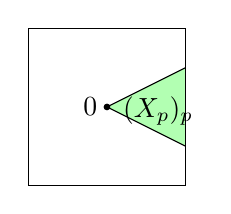
\begin{tikzpicture}[node distance=1cm]
			\coordinate (O) at (0, 0);
			\coordinate (bottomleft) at (-1, -1);
			\coordinate (topright) at (1, 1);
			\coordinate (upper) at (1, 0.5);
			\coordinate (lower) at (1, -0.5);
			
			\fill[fill=green!30] (O)--(upper)--(lower);
			
			
			\draw[] (bottomleft) rectangle (topright);
			
			
			\draw[-] (O) -- (upper);
			\draw[-] (O) -- (lower);
			
			\draw[fill=black] (0, 0) circle (1pt);
			\node[left] (Olabel) at (O) {$0$};
			
			\node[] (Clabel) at (0.65, -0.05) {$(\pazocal{X}_p)_p$};
			
			
		\end{tikzpicture} \\
		
		Polar & Dual & Polar of Polar \\
		
	\end{tabular}
	

\end{sectionbox}

\begin{sectionbox}
	\subsection{Important Convex Sets}
	\vspace{0.5em}
	\subsubsection{Levelsets, Epigraph, Hypograph}
	\vspace{0.5em}
	$f(x)$ convex $\iff$ $\text{epi}(f(x))$ convex \\
	$f(x)$ concave $\iff$ $\text{hypo}(f(x))$ convex \\
	$f(x)$ convex $\implies$ $\{\bm{x} \mid f(\bm{x}) \leq \alpha \}$ convex \\
	$\{\bm{x} \mid f(\bm{x}) \leq \alpha \}$ convex $\notimplies$ $f(x)$ convex, example: $f(\bm{x}) = -e^{x}$
	
	\subsubsection{Convex Hull}
	$\text{conv}(\pazocal{X}) = \{\bm{x} \mid \bm{x} = \sum_{i=1}^{K} \lambda_i x_i, \lambda_i \geq 0, \sum_{i=1}^{K} \lambda_i = 1\}$ \\
	
	\subsubsection{Conic Hull}
	$\text{cone}(\pazocal{X}) = \{\bm{x} \mid \bm{x} = \sum_{i=1}^{K} \lambda_i x_i, \lambda_i \geq 0 \}$ \\
	
	\subsubsection{Polytopes}
	$\pazocal{X} = \{\bm{x} \mid \bm{a_1}^\intercal\bm{x} \leq b1, \bm{a_2}^\intercal\bm{x} \leq b2\, ...\} = \{\bm{x} \mid \bm{A}\bm{x} \leq \bm{b}\}$ \\
	\subsubsection{Simplexes}
	\vspace{0.3em}
	a Polytope in $\mathbb{R}^n$ defined by $n+1$ inequalities \\
\end{sectionbox}

\begin{sectionbox}
    \subsection{Caratheodory Theorem}
	\vspace{0.3em}
	Any $\bm{x} \in \text{conv}(\pazocal{X})$ with $\bm{x} \in \mathbb{R}^n$ can be represented by a convex combination of $n+1$ points $x_i \in \pazocal{X}$ as: \\
	
	\begin{center}
		$\bm{x} = \sum_{i=1}^{n+1} \lambda_i \bm{x_i}, \bm{x_i} \in \pazocal{X}, \lambda_i \geq 0, \sum_{i=1}^{n+1} \lambda_i = 1$
	\end{center}

\end{sectionbox}

\begin{sectionbox}
	\subsection{Closest Point Theorem}
	\vspace{0.3em}
	If $\pazocal{X}$ \textbf{is convex} then there always exists a \textbf{unique} $\bm{x}^* \in \pazocal{X}$ with a minimum distance to $\bm{y} \in \mathbb{R}^n$: \\
	
	\begin{center}
		$(\bm{y} - \bm{x}^*)^\intercal(\bm{x} - \bm{x}^*) \leq 0, \forall \bm{x} \in \pazocal{X}$
	\end{center} 
	
\end{sectionbox}

\begin{sectionbox}
	\subsection{Fundamental Separation Theorem}
	\vspace{0.3em}
	(follows from Closest Point Theorem) \\
	If $\pazocal{X}$ \textbf{is convex, non-empty and closed}, then there exists a normal vector $\bm{p}$ and scalar $\alpha$ such that: \\
	
	\begin{center}
		$\bm{p}^\intercal\bm{x} > \alpha \forall x \notin \pazocal{X}$ \\
		$\bm{p}^\intercal\bm{x} \leq \alpha \forall x \in \pazocal{X}$
	\end{center}

	\textbf{Corollary:} \\
	$\pazocal{X}$ is the intersection of all closed half-spaces containing $\pazocal{X}$
	
\end{sectionbox}

\begin{sectionbox}
	\subsection{Supporting Hyperplane Theorem}
	\vspace{0.3em}
	If $\pazocal{X}$ \textbf{is convex, non-empty and closed} with $\bar{\bm{x}} \in \partial\pazocal{X}$ then there exists a hyperplane $\pazocal{H}$ defined by a normal vector $\bm{p}$ such that:
	
	\begin{center}
		$\pazocal{H} = \{ \bm{x} \mid \bm{p}^\intercal(\bm{x} - \bar{\bm{x}}) \leq 0 \forall \bm{x} \in \pazocal{X} \}$
	\end{center}

	where $\pazocal{H}$ supports $\pazocal{X}$ at $\bar{\bm{x}}$

\end{sectionbox}

\begin{sectionbox}
	\subsection{Farkas Theorem}
	\vspace{0.3em}
	(follows from Fundamental Separation Theorem) \\
	Exactly one of the following statements is true:
	\begin{center}
		\begin{enumerate}
			\item $\exists \bm{x} \in \mathbb{R}^n \mid \bm{A}\bm{x} \leq \bm{0}, \bm{c}^\intercal\bm{x} > 0$
			\item $\exists \bm{y} \in \mathbb{R}^m \mid \bm{A}^\intercal\bm{y} = \bm{c}, \bm{y} \leq \bm{0}$
		\end{enumerate}
	\end{center}
	\vspace{0.5em}
	\textbf{Geometric interpretation} \\

	\begin{tabular}{c c}
		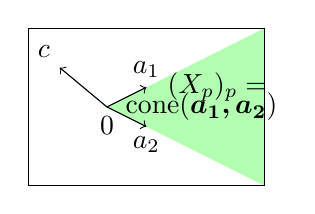
\begin{tikzpicture}[node distance=1cm]
			\coordinate (O) at (0, 0);
			\coordinate (c) at (-0.6, 0.5);
			\coordinate (a1) at (0.5, 0.25);
			\coordinate (a2) at (0.5, -0.25);
			\coordinate (bottomleft) at (-1, -1);
			\coordinate (topright) at (2, 1);
			\coordinate (bottomright) at (2, -1);
			\coordinate (cone) at (1.2, 0);
			\coordinate (ppcone) at (1.4, 0.25);
			
			\fill[fill=green!30] (O)--(topright)--(bottomright);
			
			\draw[] (bottomleft) rectangle (topright);
			
			\node[below] (Olabel) at (O) {$0$};
			
			\node[] (conelabel) at (cone) {$\text{cone}(\bm{a_1, a_2})$};
			
			\node[] (ppconelabel) at (ppcone) {$(\pazocal{X}_p)_p = $};
			
			\draw[->] (O) -- (c) node [above left] {$c$};
			\draw[->] (O) -- (a1) node [above] {$a_1$};
			\draw[->] (O) -- (a2) node [below] {$a_2$};
			
		\end{tikzpicture} &
		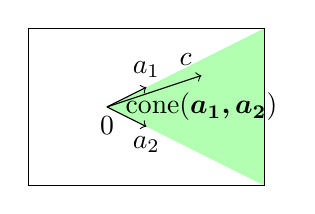
\begin{tikzpicture}[node distance=1cm]
			\coordinate (O) at (0, 0);
			\coordinate (c) at (1.2, 0.4);
			\coordinate (a1) at (0.5, 0.25);
			\coordinate (a2) at (0.5, -0.25);
			\coordinate (bottomleft) at (-1, -1);
			\coordinate (topright) at (2, 1);
			\coordinate (bottomright) at (2, -1);
			\coordinate (cone) at (1.2, 0);
			
			\fill[fill=green!30] (O)--(topright)--(bottomright);
			
			\draw[] (bottomleft) rectangle (topright);
			
			\node[below] (Olabel) at (O) {$0$};
			
			\node[] (conelabel) at (cone) {$\text{cone}(\bm{a_1, a_2})$};
			
			\draw[->] (O) -- (c) node [above left] {$c$};
			\draw[->] (O) -- (a1) node [above] {$a_1$};
			\draw[->] (O) -- (a2) node [below] {$a_2$};
			
		\end{tikzpicture} \\
	
		(1) has a solution & (2) has a solution \\
		$c \notin \text{cone}(a_1, a_2)$ & $c \in \text{cone}(a_1, a_2)$
		
	\end{tabular}
	\vspace{0.5em}
	\subsubsection{Gordan's Theorem}
	\vspace{0.5em}
	Exactly one of the following statements is true:
	\begin{center}
		\begin{enumerate}
			\item $\exists \bm{x} \in \mathbb{R}^n \mid \bm{A}\bm{x} < \bm{0}$
			\item $\exists \bm{y} \in \mathbb{R}^m \mid \bm{A}^\intercal\bm{y} = \bm{c}, \bm{y} \geq \bm{0}, \bm{y} \neq \bm{0}$
		\end{enumerate}
	\end{center}
	
\end{sectionbox}


\section{Convex Functions}

\begin{sectionbox}
	\subsection{Convexity Preserving Operations}
	\vspace{0.5em}
	The function $f(\bm{x})$ is convex if it is a...
	\begin{enumerate}
		\item \textbf{conic combination} of convex functions:
		\begin{center}
			$f(\bm{x}) = \sum_{i=1}^{K} \lambda_i f_i(\bm{x}), \lambda_i \geq 0$
		\end{center}
		
		\item composite of a \textbf{nondecreasing, univariate, convex} $g(\bm{x})$ and a \textbf{convex} $h(\bm{x})$:
		\begin{center}
			$f(\bm{x}) = g(h(\bm{x}))$
		\end{center}
		
		\item \textbf{pointwise maximum} of convex functions:
		\begin{center}
			$f(\bm{x}) = \max_{i=1,\dots,K}\{f_1(\bm{x}),\dots,f_K(\bm{x})\}$
		\end{center}
	
		\item \textbf{negative of a concave} function $g(\bm{x})$:
		\begin{center}
			$f(\bm{x}) = -g(\bm{x})$
		\end{center}
		
	\end{enumerate}
\end{sectionbox}

\begin{sectionbox}
	\subsection{Checking for convexity}
	\subsubsection{Definition of a convex function}
	\vspace{0.3em}
	A function $f(x)$ is convex if:
	\begin{center}
		$f(\lambda \bm{x_1} + (1-\lambda)\bm{x_2}) \bm{\leq} \lambda f(\bm{x_1}) + (1-\lambda) f(\bm{x_2})$ \\
		\vspace{0.2em}
		$\forall \lambda \in [0, 1]$
	\end{center}
	\vspace{0.5em}
	\subsubsection{First Order criterion}
	\vspace{0.3em}
	A $f(x)$ which is \textbf{at least once differentiable} is convex if:
	\begin{center}
		$f(\bar{\bm{x}}) \nabla f^\intercal(\bar{\bm{x}})(\bm{x} - \bar{\bm{x}}) \bm{\leq} f(\bm{x}) \qquad \forall \bm{x}, \bar{\bm{x}}$
	\end{center}
	\vspace{0.5em}
	\subsubsection{Second Order criterion}
	\vspace{0.3em}
	A $f(x)$ which is \textbf{at least twice differentiable} is convex if:
	\begin{center}
		$0 \bm{\leq} \nabla^2f(\bm{x}) \qquad \forall \bm{x}$
	\end{center}
	\vspace{0.5em}
	\textbf{Remark:} For concavity $\bm{\geq}$ must hold
\end{sectionbox}

\begin{sectionbox}
	\subsection{Quasiconvexity}
	A function $f(\bm{x})$ is quasiconvex if for a $\lambda \in (0, 1)$:
	\begin{center}
		$f(\lambda \bm{x_1} + (1-\lambda)\bm{x_2}) \leq \max\{f(\bm{x_1}), f(\bm{x_2})\}$
	\end{center}
	and strictly quasiconvex if it hold with strict equality. \\
	\textbf{Interpretation:} $f$ remains nondecreasing in an increasing direction. \\
	\textbf{Quasiconvex function may not have a unique global minimizer}
	\vspace{0.5em}
	
	\subsection{Pseudoconvexity}
	A function $f(\bm{x})$ is pseudoconvex if for $\bm{x_1}, \bm{x_2} \in \text{dom}(f)$:
	\begin{center}
		$\nabla f^\intercal(\bm{x_1})(\bm{x_2} - \bm{x_1}) \geq 0 \implies f(\bm{x_2}) \geq f(\bm{x_1})$
	\end{center}
	and strictly pseudoconvex if it holds with strict equality for $\bm{x_1} \neq \bm{x_2}$. \\
	\textbf{Interpretation:} $f$ is nondecreasing for all gradient directions. \\
	\textbf{Strict pseudoconvex functions have a unique global minimizer}
\end{sectionbox}

\section{Linear Programming}

\begin{sectionbox}
	\subsection{Extreme Points}
	$\bm{x}_{(\text{EP})} \in \pazocal{X}$ can't be represented by $\bm{x_1}, \bm{x_2} \in \pazocal{X}$ for any $\lambda \in (0, 1)$:
	\begin{center}
		$\bm{x}_{(\text{EP})} = \lambda \bm{x_1} + (1-\lambda)\bm{x_2} \quad \implies \quad \bm{x}^{(\text{EP})} = \bm{x_1} = \bm{x_2}$ 
	\end{center}
	\textbf{Interpretation:} Corner points or curve borders of a convex compact set.
	\vspace{0.5em}
	
	\subsection{Extreme Directions}
	$\bm{d}_{(\text{ED})}$ can't be represented by a positive linear combination of directions:
	\begin{center}
		$\bm{d}_{(\text{ED})} = \lambda_1 \bm{d_1} + \lambda_2 \bm{d_2} \quad \implies \quad \bm{d_1} = \alpha\bm{d_2}$ \\
		$\lambda_1, \lambda_2, \alpha > 0$
	\end{center}
	\textbf{Interpretation:} Direction in which the set is unbounded.
	\vspace{0.5em}
	
	\subsection{Polyhedral Sets (Polyhedron)}
	Intersection of half-spaces, \textbf{always closed and convex}. \\
	\vspace{0.3em}
	\textbf{Primal Standard Form}
	\begin{center}
		$\pazocal{X} = \{\bm{x} \in \mathbb{R}^n \mid \bm{A}\bm{x} = \bm{b}, \bm{x} \geq 0 \}$
	\end{center}
	\textbf{ Dual Standard Form}
	\begin{center}
		$\pazocal{X} = \{\bm{x} \in \mathbb{R}^n \mid \bm{A}\bm{x} \leq \bm{b}\}$
	\end{center}
	\vspace{0.5em}

	\subsection{EPs and EDs of Polyhedra}
	\textbf{Requirements for EPs: } $\bm{A} \in \mathbb{R}^{m \times n}$, $\text{rank}(\bm{A}) = m$ and $n \geq m$
	\begin{center}
		$\bm{A}\bm{x} = \begin{bmatrix}
			\bm{B} & \bm{N}
		\end{bmatrix} \begin{bmatrix}
		\bm{x_B} \\
		\bm{x_N}
	\end{bmatrix}, \quad \bm{B} \in \mathbb{R}^{m \times m}, \bm{N} \in \mathbb{R}^{m \times (n-m)}$
	\end{center}
	\textbf{Extreme point:}
	\begin{center}
		$\bm{x}_{(\text{EP})} = \begin{bmatrix}
			\bm{B}^{-1}\bm{b} \\
			\bm{0}_{n-m}
		\end{bmatrix} \geq \bm{0}$
	\end{center}
	\textbf{Extreme direction:}
	\begin{center}
		$\bm{d}_{(\text{ED})} =  \begin{bmatrix}
			-\bm{B}^{-1}\bm{N}\bm{e_j} \\
			\bm{e_j}
		\end{bmatrix}  \geq \bm{0}$
	\end{center}
	\textbf{Finding all EPs and EDs:} \\
	There are \textbf{at most} $\binom{n}{m}$ EPs and \textbf{at most} $(n-m)\binom{n}{m}$ EDs. \\
	Permute Problem with $\bm{\Pi}$ with $\bm{\Pi}^\intercal\bm{\Pi} = \bm{I}$:
	\begin{center}
		$\bm{A}\bm{x} = \bm{A}\bm{\Pi}\bm{\Pi}^\intercal\bm{x} = \bm{A}^{\Pi}\bm{x}^{\Pi}$
	\end{center}
	Example permutation: $\bm{a}_i$ is the i-th column of $\bm{A}$ \\
	\begin{center}
		$\begin{bmatrix}
			\bm{a_1} & \bm{a_2} & \bm{a_3}
		\end{bmatrix} \begin{bmatrix}
			0 & 1 & 0 \\
			1 & 0 & 0 \\
			0 & 0 & 1
	\end{bmatrix} = \begin{bmatrix}
	\bm{a_2} & \bm{a_1} & \bm{a_3}
\end{bmatrix}$
	\end{center}
	
\end{sectionbox}

\begin{sectionbox}
	\subsection{Linear Programs}
	\textbf{Standard Form:}
	\begin{center}
		$\min\limits_{\bm{x}} \bm{c}^\intercal\bm{x} \qquad \text{s.t.} \quad \bm{A}\bm{x}=\bm{b}, \quad \bm{x}\geq\bm{0}$
	\end{center}
	\textbf{LP is bounded if:}
	\begin{center}
		$\bm{c}^\intercal\bm{d}^{(\text{ED})}_j \geq 0 \qquad \forall j$
	\end{center}
	\textbf{Optimizer} of a LP is an EP:
	\begin{center}
		$\bm{x}^* = \argmin\limits_{\bm{x}^{(\text{EP})}}\{\bm{c}^\intercal\bm{x}^{(\text{EP})}_i\} \qquad \forall i$
	\end{center}
	LPs are always \textbf{convex} OPs. \\
	
\end{sectionbox}

\begin{sectionbox}
	\subsection{Simplex Algorithm}
	\textbf{Solve Linear Program of the form}
	\begin{emphbox}
		$\min\limits_{\bm{x}} \bm{c}^\intercal\bm{x} \quad \text{s.t. } \bm{A}\bm{x} = \bm{b}, \quad \bm{x}\geq \bm{0}$
	\end{emphbox}
	\vspace{0.5em}
	\textbf{0 Find EP:} \\
	\begin{center}
		$\bm{A}^{\Pi} = \bm{A}\bm{\Pi} = \begin{bmatrix}
			\bm{B} & \bm{N}
		\end{bmatrix}, \bm{x}^{\Pi}_{\text{EP}} = \begin{bmatrix}
			\bm{B}^{-1}\bm{b} \\ \bm{0}
		\end{bmatrix} \geq \bm{0}$ \\
		$\bm{c}^{\Pi} = \begin{bmatrix}
			\bm{c_B} \\ \bm{c_N}
		\end{bmatrix}$
	\end{center}
	\vspace{1em}
	
	\textbf{1 Check criterium for optimality}
	\begin{emphbox}
		$\bm{c_B}^\intercal\bm{B}^{-1}\bm{N}-\bm{c_N}^\intercal \leq \bm{0}$ ?
	\end{emphbox}
	\begin{itemize}
		\item[] yes $\implies$ $\bm{x}^* = \bm{x_{\text{EP}}} = \bm{\Pi}\bm{x_{\text{EP}}^{\Pi}}$
		\item[] no $\implies$ continue
	\end{itemize}
	\vspace{1em}
	
	\textbf{2 Find direction to next EP}
	\begin{emphbox}
		$j = \argmax\{[\bm{c_B}^\intercal\bm{B}^{-1}\bm{N}-\bm{c_N}^\intercal]_{i}\}$ \\
		$\bm{B}^{-1}\bm{N}\bm{e_j} \leq 0$ ?
	\end{emphbox}
	\begin{itemize}
		\item[] yes $\implies$ LP unbounded
		\item[] no $\implies$ continue
	\end{itemize}
	\vspace{1em}
	
	\textbf{3 Compute new permuted EP}
	\begin{center}
		$\bm{d}^{\Pi} = \begin{bmatrix}
			-\bm{B}^{-1}\bm{N}\bm{e_j} \\
			\bm{e_j}
		\end{bmatrix}$ \\
		\vspace{0.5em}
		$\bm{x}^{\Pi}_{\text{EP,new}} = \bm{x}^{\Pi}_{\text{EP}} + \lambda_{\text{max}}\bm{d}^{\Pi} \bm{\geq} \bm{0}$ \\
		\vspace{0.5em}
		$i = \argmin\{[\lambda_{\text{max}}\bm{d}^{\Pi}]_{j}\}$ \\
		\textit{(index in $\bm{x}^{\Pi}_{\text{EP}}$ that limits $\lambda_{\text{max}}$)}
	\end{center}
	\vspace{1em}
	
	\textbf{4 Compute new Permutation Matrix and go to step 0}
	\begin{center}
		$\bm{x}_{\text{EP, new}} = \bm{\Pi}\bm{x}^{\Pi}_{\text{EP, new}}$ \\
		\vspace{0.5em}
		Choose $\bm{\Pi}_{\text{new}}$ such that $i$ is nonbasic and $j$ is basic.
	\end{center}
	\vspace{4em}
	
	\subsubsection{Degeneracy}
	\vspace{0.3em}
	Theoretical infinite loop (\textit{cycling}) if:
	\begin{center}
		$[\bm{x_B}]_{i} = 0 \quad \implies \quad \lambda_{\text{max}}=0$
	\end{center}
	

\end{sectionbox}

\begin{sectionbox}
	\textbf{Binominalcoefficient: } \\
	\begin{center}
		$\binom{n}{m} = \frac{n!}{m!(n-m)!}$
	\end{center}
\end{sectionbox}

\section{Optimality Conditions}

\begin{sectionbox}
	\subsection{Unconstrained Optimization}
	\subsubsection{First Order}
	Sufficient if $f(\bm{x})$ \textbf{pseudoconvex} at $\bm{x}^*$. $\bm{x}^*$ is \textbf{global} minimizer
	\begin{center}
		$\nabla f(\bm{x}^*) = 0$
	\end{center}
	\vspace{0.5em}
	\subsubsection{Second Order}
	Always sufficient. $\bm{x}^*$ is \textbf{local} minimizer
	\begin{center}
		$\nabla f(\bm{x}^*) = 0 \qquad \textbf{and} \qquad \nabla^2 f(\bm{x}^*) \quad \text{pdf}$
	\end{center}
\end{sectionbox}

\begin{sectionbox}
	\subsection{Geometric Optimality Conditions}
	\vspace{0.3em}
	\textbf{Cone of feasible directions}
	\begin{center}
		$\pazocal{G}_0(\bm{x}^*) = \{\bm{d} \mid \nabla g_i^\intercal(\bm{x}^*)\bm{d} < 0 \forall i \in \pazocal{I}(\bm{x}^*) \}$
	\end{center}
	\textbf{Cone of improving directions}
	\begin{center}
		$\pazocal{F}_0(\bm{x}^*) = \{\bm{d} \mid \nabla f^\intercal(\bm{x}^*)\bm{d} < 0 \}$
	\end{center}
	\textbf{Sufficient condition} for a \textit{local} minimizer if $f(\bm{x})$ is pseudoconvex, $g_i(\bm{x})$ strictly pseudoconvex at $\bm{x}^*$
	\begin{center}:
		$\pazocal{G}_0(\bm{x}^*) \cap \pazocal{F}_0(\bm{x}^*) = \emptyset$
	\end{center}
	\vspace{1em}
\end{sectionbox}

\begin{emphbox}
	\textbf{Generic constrained OP:}
	\begin{align}
		\min_{\bm{x}} f(\bm{x}) \qquad \text{s.t.} \quad & g_i(\bm{x}) \leq 0, \forall i \in \{1, \dots, l\} \notag\\
		& h_i(\bm{x}) = 0, \forall j \in \{1, \dots, m\} \notag
	\end{align}
\end{emphbox}

\begin{sectionbox}
	\subsection{Fritz John Optimality Conditions}
	\begin{center}
		$u_0 \nabla f(\bm{x}^*) + \sum\limits_{i \in \pazocal{I}(\bm{x}^*)}^{} u_i\nabla g_i(\bm{x}^*) + \sum\limits_{j=1}^{m} v_j \nabla h_j(\bm{x}^*) = 0$ \\
		$u_0 \geq 0$, $u_i \geq 0$
	\end{center}

	\textbf{Necessary} if:
	\begin{itemize}
		\item $f(\bm{x})$ and $g_i(\bm{x})$ $\forall i \in \pazocal{I}(\bm{x}^*)$ differentiable at $\bm{x}^*$
		\item $g_i(\bm{x})$ $\forall i \notin \pazocal{I}(\bm{x}^*)$ continuous at $\bm{x}^*$
		\item $h_j(\bm{x})$ $\forall j \in \{1, \dots, m\}$ continuously differentiable at $\bm{x}^*$
	\end{itemize}
	\textbf{Sufficient} if:
	\begin{itemize}
		\item $h_j(\bm{x})$ $\forall j \in \{1, \dots, m\}$ affine
		\item $\nabla h_j(\bm{x})$ $\forall j \in \{1, \dots, m\}$ linearly independent
		\item $f(\bm{x})$ pseudoconvex over $\pazocal{U}(\bm{x}^*) \cap \pazocal{S}(\bm{x}^*)$
		\item $g_i(\bm{x})$ $\forall i \notin \pazocal{I}(\bm{x}^*)$ strictly pseudoconvex over $\pazocal{U}(\bm{x}^*) \cap \pazocal{S}(\bm{x}^*)$
	\end{itemize}
	\textbf{Problems} :
	\begin{itemize}
		\item $u_0 = 0$ allowed $\implies$ ignores objective
		\item $\pazocal{I}(\bm{x})$ requires determining active constraints
		\item[] $\implies$ KKT resolves these issues with $u_0 = 1$ and CS
	\end{itemize}
	
\end{sectionbox}

\begin{sectionbox}
	\subsection{KKT Optimality Conditions}
	\begin{emphbox}
		\textbf{Primal Feasibility (PF)}: \\
		\vspace{0.3em}
		$g_i(\bm{x}) \leq 0, \forall i \in \{1, \dots, l\}$ \\
		$h_i(\bm{x}) = 0, \forall j \in \{1, \dots, m\}$ \\
		\vspace{1em}
		\textbf{Dual Feasibility (DF)}: \\
		$\nabla f(\bm{x}) + \sum\limits_{i=1}^{l} u_i\nabla g_i(\bm{x}) + \sum\limits_{j=1}^{m} v_j\nabla h_j(\bm{x}) = \bm{0}$ \\
		$u_i \geq 0$ $\forall i \in \{1, \dots, l\}$ \\
		\vspace{1em}
		\textbf{Complementary Slackness (CS)}: \\
		\vspace{0.3em}
		$u_i g_i(\bm{x}) = 0$ $\forall i \in \{1, \dots, l\}$
	\end{emphbox}

	\textbf{Necessary} if:
	\begin{itemize}
		\item $f(\bm{x})$ and $g_i(\bm{x})$ $\forall i \in \pazocal{I}(\bm{x}^*)$ differentiable at $\bm{x}^*$
		\item $g_i(\bm{x})$ $\forall i \notin \pazocal{I}(\bm{x}^*)$ continuous at $\bm{x}^*$
		\item $h_j(\bm{x})$ $\forall j \in \{1, \dots, m\}$ continuously differentiable at $\bm{x}^*$
		\item $\nabla g_i(\bm{x}^*)$ $\forall i \in \pazocal{I}(\bm{x}^*)$ and $\nabla h_j(\bm{x}^*)$ $\forall j \in \{1, \dots, m\}$ linearly independet
	\end{itemize}

	\textbf{Sufficient} if:
	\begin{itemize}
		\item $f(\bm{x}^*)$ pseudoconvex and active $g_i(\bm{x}^*)$ quasiconvex
		\item $h_j(\bm{x}^*)$ quasiconvex $\forall j \mid v_j > 0$
		\item $h_j(\bm{x}^*)$ quasiconcave $\forall j \mid v_j < 0$
	\end{itemize}

\end{sectionbox}

\begin{sectionbox}
	\subsection{Constraint Qualifications}
	KKT conditions are \textbf{necessary} if at least one CQ is satisfied
	\subsubsection{Linear Independence Constraint Qualification}
	\vspace{0.3em}
	\begin{itemize}
		\item inactive $g_i$ are continuous at $\bm{x}^*$
		\item $h_j$ $\forall j \in \{1, \dots, m\}$ are continuously differentiable at $\bm{x}^*$
		\item active $\nabla g_i(\bm{x}^*)$ and $\nabla h_j(\bm{x}^*)$ are linearly independent
	\end{itemize}
	\vspace{1em}
	\subsubsection{Slater's Constraint Qualification}
	\vspace{0.3em}
	\begin{itemize}
		\item active $g_i$ are pseudoconvex at $\bm{x}^*$
		\item inactive $g_i$ are continuous at $\bm{x}^*$
		\item $h_j$ are pseudoconvex, pseudoconcave and continuously differentiable at $\bm{x}^*$
		\item $\nabla h_j$ are linearly independent
		\item $\pazocal{X}$ \textbf{has an interior point}
	\end{itemize}
	\vspace{0.5em}
	KKT conditions are \textbf{sufficient} if: \\
	... the \textbf{OP is convex} (e.g. LPs) \\
	... OR Slater CQs + $f(\bm{x})$ \textbf{pseudoconvex}
\end{sectionbox}

\section{Lagrangian Duality}

\begin{sectionbox}
	\subsection{Lagrangian Dual Problem}
	\begin{emphbox}
		\textbf{Lagrangian function} \\
		\vspace{0.3em}
		$\phi(\bm{x}, \bm{u}, \bm{v}) = f(\bm{x}) + \bm{u}^\intercal\bm{g}(\bm{x}) + \bm{v}^\intercal\bm{h}(\bm{x})$ \\
		\vspace{1em}
		\textbf{Dual function} \\
		\vspace{0.3em}
		$\theta(\bm{u}, \bm{v}) = \inf\limits_{\bm{x} \in \pazocal{S}} \{ \phi(\bm{x}, \bm{u}, \bm{v}) \}$ \\
		\vspace{1em}
		\textbf{Dual Problem} \\
		\vspace{0.3em}
		$\max\limits_{\bm{u}, \bm{v}} \quad \theta(\bm{u}, \bm{v}) \qquad \text{s.t.} \quad \bm{u} \geq \bm{0}$
	\end{emphbox}

	The D-OP is \textbf{always convex and not unique}. \\
	The dual function $\theta$ is always concave and may not be differentiable.

\end{sectionbox}

\begin{sectionbox}
	\subsection{Geometric Interpretation of the D-OP}
	D-OP for Problem with single IEQ:
	\begin{center}
		$\max\limits_{\bm{u} \leq \bm{0}} \inf\limits_{\bm{x}} \{f(\bm{x}) + ug(\bm{x})\}$
	\end{center}
	Reformulate to get a linear expression:
	\begin{center}
		$\alpha := f(\bm{x}) + ug(\bm{x}) := z + uy$ \\
		$z = \alpha - uy$
	\end{center}
	where $-u$ defines the slope which is always $\leq 0$. \\
	\\
	\begin{tabular}{c@{\hspace{5mm}}@{\extracolsep\fill}c@{\hspace{5mm}}@{\extracolsep\fill}c}
		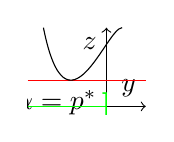
\begin{tikzpicture}[node distance=1cm]
			\coordinate (O) at (0, 0);
			\coordinate (bottomleft) at (-1, -0.1);
			\coordinate (topright) at (0.5, 1);
			
			\clip (bottomleft) rectangle (topright);
			
			\draw[->] (-1, 0) -- (0.5, 0) node[above left] {$y$};
			\draw[->] (0, -0.1) -- (0, 1) node[below left] {$z$};
			
			\draw[-, color=red] (-1, 0.33) -- (0.5, 0.33);
			\node[below left] (alabel) at (0, 0.33) {$\alpha = p^*$};
			
			\draw (-0.8,1) .. controls (-0.5, -0.5) and (0, 1) .. (0.2, 1);
			
			\node[color=green] (tInv) at (O) {$\bm{]}$};
			\draw[-, color=green] (-1, 0) -- (0, 0);
			
		\end{tikzpicture} &
		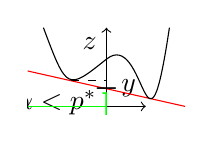
\begin{tikzpicture}[node distance=1cm]
			\coordinate (O) at (0, 0);
			\coordinate (bottomleft) at (-1, -0.1);
			\coordinate (topright) at (1, 1);
			
			\clip (bottomleft) rectangle (topright);
			
			\draw[->] (-1, 0) -- (0.5, 0) node[above left] {$y$};
			\draw[->] (0, -0.1) -- (0, 1) node[below left] {$z$};
			
			\draw[-, color=red] (-1, 0.45) -- (1, 0);
			\node[] (amark) at (0, 0.23) {$\bm{-}$};
			\node[below left] (alabel) at (0, 0.33) {$\alpha < p^*$};
			\draw[dashed] (-0.45, 0.33) -- (0, 0.33);
			
			\draw 	(-0.8, 1) .. controls (-0.5, 0.2) .. 
			(0, 0.6) .. controls (0.5, 1) and (0.5, -1) .. (0.8, 1);
			
			\node[color=green] (tInv) at (O) {$\bm{]}$};
			\draw[-, color=green] (-1, 0) -- (0, 0);
			
		\end{tikzpicture}
		 &
		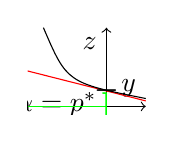
\begin{tikzpicture}[node distance=1cm]
			\coordinate (O) at (0, 0);
			\coordinate (bottomleft) at (-1, -0.1);
			\coordinate (topright) at (0.5, 1);
			
			\clip (bottomleft) rectangle (topright);
			
			\draw[->] (-1, 0) -- (0.5, 0) node[above left] {$y$};
			\draw[->] (0, -0.1) -- (0, 1) node[below left] {$z$};
			
			\draw[-, color=red] (-1, 0.45) -- (0.5, 0.07);
			\node[] (amark) at (0, 0.2) {$\bm{-}$};
			\node[below left] (alabel) at (0, 0.3) {$\alpha = p^*$};
			
			\draw 	(-0.8, 1) .. controls (-0.5, 0.3) .. (0.5, 0.1);
			
			\node[color=green] (tInv) at (O) {$\bm{]}$};
			\draw[-, color=green] (-1, 0) -- (0, 0);
			
		\end{tikzpicture} \\
		$g(x)$ inactive & $g(x)$ inactive & $g(x)$ active \\
		zero gap & nonzero gap & zero gap
	\end{tabular}
\end{sectionbox}

\begin{sectionbox}
	\subsection{Weak and Strong Duality}
	
	\begin{emphbox}
		\textbf{Weak Duality} \\
		\vspace{0.3em}
		$d^* \leq p^*$
	\end{emphbox}
	Weak duality always holds \\
	\begin{emphbox}
		\textbf{Strong Duality} \\
		\vspace{0.3em}
		$d^* = p^*$
	\end{emphbox}
	Strong duality holds if:
	\begin{itemize}
		\item OP is linear
		\item or OP is convex and QC hold
	\end{itemize}
	
\end{sectionbox}

\begin{sectionbox}
	\subsection{Saddle Point Property}
	\vspace{0.3em}
	Fulfilled by $(\bm{x}^*, \bm{u}^*, \bm{v}^*)$ if strong duality holds:
	\vspace{0.5em}
	\begin{center}
		$\sup\limits_{\bm{x}} \inf\limits_{\bm{y}} f(\bm{x}, \bm{y}) \leq \inf\limits_{\bm{y}}\sup\limits_{\bm{x}} f(\bm{x}, \bm{y})$
	\end{center}
\end{sectionbox}

\begin{sectionbox}
	\subsection{Boundedness of D-OPs}
	\textbf{P-OP} is never unbounded from above \\
	\textbf{D-OP} is never unbounded from below \\
	\begin{tabular}{|c|c|c|c|}
		\hline
		\diagbox{Dual}{Primal} & finite & unbounded & infeasible \\
		\cline{1-4}
		finite & \cmark & \xmark & \xmark \\
		\cline{1-4}
		unbounded & \xmark & \xmark & \cmark \\
		\cline{1-4}
		infeasible & \xmark & \cmark & \cmark \\
		\hline
	\end{tabular}
	
\end{sectionbox}

\section{Concepts of Algorithms}

\begin{sectionbox}
	\subsection{Algorithmic Map}
	A point-to-point or point-to-set map to generate a new iterate $\bm{x}^{\text{(k+1)}}$ from $\bm{x}^{\text{(k)}}$ \\
	\begin{center}
		$\bm{A} : \pazocal{S} \implies \pazocal{S}$
	\end{center}
	\vspace{0.5em}
	
	\subsection{Solution Sets}
	The algorithm terminates if $\bm{x}^{\text{(k+1)}} \in \Omega \subset \pazocal{S}$. Possible solution sets $\Omega$:
	\begin{itemize}
		\item[] $\Omega = \{\bar{\bm{x}} \mid \bar{\bm{x}} \text{is a local miminizer} \}$
		\item[] $\Omega = \{\bar{\bm{x}} \in \pazocal{X} \mid f(\bar{\bm{x}}) \leq c \}$ with threshold $c$
		\item[] $\Omega = \{\bar{\bm{x}} \mid \bar{\bm{x}} \text{is a KKT point}\}$
	\end{itemize}
	\vspace{0.5em}

	\subsection{Stopping Criteria}
	\textbf{Error-based:}
	\begin{center}
		$\|\bm{x}^{\text{(k+1)}} - \bm{x}^{\text{(k)}} \| < \epsilon$
	\end{center}
	\textbf{Residual-based:}
	\begin{center}
		$\alpha(\bm{x}^{\text{(k)}}) - \alpha(\bm{x}^{\text{(k+1)}}) < \epsilon$
	\end{center}
	with descent function $\alpha$
	\vspace{0.5em}
	
	\subsection{Convergence Analysis}
	\textbf{Order of Convergence}
	\begin{center}
		$\lim\limits_{k \implies \infty}\sup \frac{\|\bm{x}^{\text{(k+1)}} - \bm{x}^{(\infty)}  \|_2}{\| \bm{x}^{\text{(k)}} - \bm{x}^{(\infty)} \|_2^p} = \beta < \infty$
	\end{center}
	with convergence ratio $\beta$ and order of convergence $\sup p$.
	\begin{enumerate}
		\item $p=1$ and $\beta=1$: sublinear convergence
		\item $p=1$ and $\beta \in (0, 1)$: linear convergence
		\item $p=1$ and $\beta=0$: superlinear convergence
		\item $p=2$ and $\beta < \inf$: superlinear convergence with quadratic order
	\end{enumerate} 
\end{sectionbox}

\section{Unconstrained Optimization}

\begin{sectionbox}
	\subsection{Bisection Algorithm}
	\vspace{0.3em}
	\begin{itemize}
		\item The function $f(\bm{x})$ \textbf{must be pseudoconvex} and once differentiable
		\item Requires initial guess for interval $\bm{x}^* \in [a^{(1)}, b^{(1)}]$
		\item Requires $n$ steps for accuracy $\epsilon$ such that:
	\end{itemize}
	\begin{center}
		$2^n \leq \frac{b^{(1)}-a^{(1)}}{\epsilon}$
	\end{center}
	\textbf{0 Initialization}:
	\begin{center}
		$\pazocal{I}^{\text{(k)}} = [a^{\text{(k)}}, b^{\text{(k)}}] \gets a, b \mid x^* \in [a, b], \quad a < b$
	\end{center}
	\textbf{1 Interval Center}:
	\begin{center}
		$x^{\text{(k)}} \gets \frac{a^{\text{(k)}}-b^{\text{(k)}}}{2}$
	\end{center}
	\textbf{2 Derivative at Center}:
	\begin{center}
		$f'(x^\text{(k)}) \gets \frac{\partial f(x)}{\partial x} \bigg\rvert_{x=x^{\text{(k)}}}$
	\end{center}
	\textbf{3 Check derivative sign}:
	\begin{center}
		$f'(x^\text{(k)}) \bm{<} 0 \implies \pazocal{I}^{\text{(k+1)}} = [x^{\text{k}}, b^{\text{k}}]$ \\
		$f'(x^\text{(k)}) \bm{>} 0 \implies \pazocal{I}^{\text{(k+1)}} = [a^{\text{k}}, x^{\text{k}}]$ \\
		$f'(x^\text{(k)}) \bm{=} 0 \implies x^* = x^{\text{(k)}}$
	\end{center}
	\textbf{4 Repeat until $b^{\text{(k)}} - a^{\text{(k)}} < \epsilon$}
	
\end{sectionbox}

\begin{sectionbox}
	\subsection{Newton Algorithm}
	\vspace{0.3em}
	\begin{itemize}
		\item The function $f(\bm{x})$ must be \textbf{twice differentiable}
		\item \textbf{Convergence not guaranteed} for arbitrary $\bm{x}^{\text{(0)}}$
		\item Good convergence if $\bm{x}^{\text{(0)}}$ close to $\bm{x}^*$
		\item Numerical problems if $\nabla^2f(\bm{x}^{\text{(k)}}) = 0$ (no inverse of hessian)
		\item \textbf{Convergence Independent of linear transformations}
		\item Finds $\bm{x}^*$ in one step if $f(\bm{x})$ is quadratic
	\end{itemize}
	\begin{emphbox}
		\textbf{Newton Update}:
		\begin{center}
			$\bm{x}^{\text{(k+1)}} = \bm{x}^{\text{(k)}} - \bm{H}(\bm{x}^{\text{(k)}})^{-1}\nabla f(\bm{x}^{\text{(k)}})$
		\end{center}
	\end{emphbox}
	\textbf{Newton Step}:
	\begin{center}
		$\Delta \bm{x}^{\text{(k)}} = -\bm{H}(\bm{x}^{\text{(k)}})^{-1}\nabla f(\bm{x}^{\text{(k)}})$
	\end{center}
	with
	\begin{center}
		$\nabla f^\intercal(\bm{x}^{\text{(k)}})\Delta\bm{x}^{\text{(k)}} < 0 \implies$ descent direction
	\end{center}
	\textbf{Newton Decrement}: Useful as termination criterion
	\begin{center}
		$\lambda(\bm{x}^{\text{(k)}}) = \big( \Delta {\bm{x}^{\text{(k)}}}^\intercal \bm{H}(\bm{x}^{\text{(k)}}) \Delta \bm{x}^{\text{(k)}} \big)$
	\end{center}
\end{sectionbox}

\begin{sectionbox}
	\subsection{Armijo's Stepsize Rule}
	\begin{itemize}
		\item \textit{Choose stepsize $\lambda^{\textit{(k)}}$ not too small or too large}
		\item Tuning parameters $\epsilon \in (0, 1)$ and $\alpha > 1$
	\end{itemize}
	\textbf{Line Search Function}:
	\begin{center}
		$\theta(\lambda) = f(\bar{\bm{x}} + \lambda \bm{d})$
	\end{center}
	\textbf{First Order Approximation} at $\lambda = 0$:
	\begin{center}
		$\hat{\theta}(\lambda) = \theta(0) + \lambda\epsilon\theta'(0)$
	\end{center}

	\begin{tabular}{c c}
			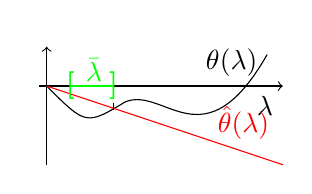
\begin{tikzpicture}[node distance=1cm]
			\coordinate (O) at (0, 0);
			\coordinate (bottomleft) at (-0.1, -1);
			\coordinate (topright) at (3, 0.5);
			
			\draw[->] (0, -1) -- (0, 0.5) node[above left] {};
			\draw[->] (-0.1, 0) -- (3, 0) node[below left] {$\lambda$};
			
			
			\draw 	(0, 0) .. controls (0.5, -0.5) ..
			(1, -0.2) .. controls (1.5, 0) and (2, -1) .. (2.8, 0.4);
			
			\draw[-, color=red] (0, 0) -- (3, -1);
			\node[above, text=red] (approxlabel) at (2.5, -0.8) {$\hat{\theta}(\lambda)$};
			\node[] (origlabel) at (2.35, 0.3) {$\theta(\lambda)$};
			
			\draw[dashed] (0.85, 0) -- (0.85, -0.3);
			\draw[-, color=green] (0.3, 0) -- (0.85, 0);
			
			\node[color=green] (lINF) at (0.3, 0) {$\bm{[}$};
			\node[color=green] (uINF) at (0.85, 0) {$\bm{]}$};
			\node[text=green] (lamlabel) at (0.6, 0.2) {$\bar{\lambda}$};
			
		\end{tikzpicture} &
		\begin{tabular}{c}
			Not too large: \\
			$\theta(\bar{\lambda}) \leq \bar{\theta}(\bar{\lambda})$ \\
			Not too small: \\
			$\theta(\alpha\bar{\lambda}) > \bar{\theta}(\alpha\bar{\lambda})$
		\end{tabular}
	\end{tabular}
	
\end{sectionbox}

\pagebreak

\section{Solution Methods for Dual Problems}

\begin{sectionbox}
	\subsection{Possible Advantages}
	\begin{itemize}
		\item reduction in problem complexity
		\item decoupling into smaller problems
	\end{itemize}
\end{sectionbox}

\begin{sectionbox}
	\subsection{Subgradients}
	\begin{emphbox}
		\textbf{Subgradient $\xi$ of \underline{convex} $f(\bm{x})$ at $\bar{\bm{x}}$}: \\
		\vspace{0.3em}
		$f(\bm{x}) \bm{\geq} f(\bar{\bm{x}}) + \xi^\intercal(\bm{x} - \bar{\bm{x}})$
	\end{emphbox}
	\begin{emphbox}
		\textbf{Subgradient $\xi$ of \underline{concave} $\theta(\bm{u})$ at $\bar{\bm{u}}$}: \\
		\vspace{0.3em}
		$\theta(\bm{u}) \bm{\leq} \theta(\bar{\bm{u}}) + \xi^\intercal(\bm{u} - \bar{\bm{u}})$
	\end{emphbox}

	\subsection{Subdifferential}
	\textbf{Convex set} of all subgradients for \textbf{\underline{concave}} $\theta(\bar{\bm{u}})$:
	\vspace{0.3em}
	\begin{center}
		$\partial \theta(\bar{\bm{u}}) = \text{conv}(\{ \xi \mid \theta(\bm{u}) \bm{\leq} \theta(\bar{\bm{u}}) + \xi^\intercal(\bm{u} - \bar{\bm{u}}) \forall \bm{u} \in \pazocal{U} \})$
	\end{center}
	is a singleton if $\theta(\bm{u})$ is differentiable at $\bar{\bm{u}}$.

\end{sectionbox}

\begin{sectionbox}
	\subsection{Subgradient Methods}
	\vspace{0.3em}
	\begin{itemize}
		\item $\theta(\bm{u}, \bm{v})$ not always differentiable $\implies$ use subgradients
		\item subgradients not always ascent directions
		\item Stepsize control necessary
	\end{itemize}
	\vspace{0.5em}
	
	\textbf{0 Start with Candidate Point } $\bm{u}^{\text{(k)}}$ \\
	\vspace{0.5em}
	
	\textbf{1 Get primal variables } $\bm{x}^{\text{(k)}}$ \\
	\begin{center}
		$\bm{x}^{\text{(k)}} = \argmin\limits_{\bm{x}} \phi(\bm{x}, \bm{u}^{\text{(k)}})$
	\end{center}
	\vspace{0.5em}
	
	\textbf{2 Calculate subgradient } $\bm{\xi}^{\text{(k)}}$ \\
	\begin{center}
		$\bm{\xi}^{\text{(k)}} = \bm{g}(\bm{x}^{\text{(k)}})$
	\end{center}
	\vspace{0.5em}
	
	\textbf{3 Update dual variables } \\
	\begin{emphbox}
		\begin{center}
			$\bm{u}^{\text{(k+1)}} = \bm{P}_{\pazocal{U}} \big( \bm{u}^{\text{(k)}} \pm s^{\text{(k)}}\bm{\xi}^{\text{(k)}} \big)$
		\end{center}
		with \textbf{$\bm{+}$ for concave} and \textbf{$\bm{-}$ for convex} \\
		and $\bm{P}_{\pazocal{U}}$ projects new iterate into feasible set $\pazocal{U}$. \\
	\end{emphbox}
	
	\textbf{Optimal Stepsize} (practically unknown, requires $\bm{u}^*$):
	\begin{center}
		$s^{\text{(k)}} = \frac{\theta(\bm{u}^*) - \theta(\bm{u}^{\text{(k)}})}{\| \bm{\xi}^{\text{(k)}} \|_2^2}$
	\end{center}
	\vspace{0.5em}
	
	\textbf{Constant Stepsize}
	\begin{center}
		$s^{\text{(k)}} = s > 0 \quad \forall k$
	\end{center}
	\begin{itemize}
		\item[] Bounded norm of subgradient $\| g(\bm{x}^{\text{(k)}}) \|_2 < C$
		\item[] At best, $\theta(\bm{u}^{\text{(k)}}) \leq \theta(\bm{u}^*) - s\frac{C^2}{2} = d^* - s\frac{C^2}{2}$
	\end{itemize}
	\vspace{0.5em}
	
	\textbf{Diminishing Stepsize}
	\begin{center}
		$s^{\text{(k)}} > 0, \quad \lim\limits_{k \implies \infty} s^{\text{(k)}} = 0, \quad \sum\limits_{k}^{\infty} s^{\text{(k)}} = \infty$
	\end{center}
	Convergence of $\bm{u}^{\text{(k)}} \implies \bm{u}^*$ only guaranteed if $\bm{g}(\bm{x}^{\text{(k)}})$ bounded and additionally:
	\begin{center}
		$\sum\limits_{k=1}^{\infty} (s^{\text{(k)}})^2 < \infty$
	\end{center}
	\vspace{0.5em}
\end{sectionbox}


\begin{sectionbox}
	\subsection{Cutting Plane Algorithm}
	\begin{itemize}
		\item approximate $\theta(\bm{u}, \bm{v})$ by finite number of hyperplanes
		\item Outer approximation: $\theta(\bm{u}^*, \bm{v}^*) = d^* \leq z^{\text{(k)}}$
		\item First MP may be unbounded if $\bm{x}^{\text{(0)}}$ is not strictly feasible
	\end{itemize}
	\begin{emphbox}
		\textbf{Lower Bound on $d^*$} \\
		\vspace{0.3em}
		$y^{\text{(k)}} = \max\limits_{j=1,\dots,k} \theta(\bm{u}^{\text{(j)}}) \quad \leq \quad d^*$ \\
		\textit{Smallest value among all current supporting points $\bm{u}^{\text{(j)}}$}
	\end{emphbox}
	\begin{emphbox}
		\textbf{Upper Bound on $d^*$} \\
		\vspace{0.3em}
		$z^{\text{(k)}} \quad \geq \quad d^*$ \\
		\textit{Solution to current master program, outer approximation}
	\end{emphbox}

	\textbf{ 0 Initialization}: \\
	 Interior point $\bm{x}^{\text{(0)}} \iff \bm{g}(\bm{x}^{(0)}) < 0 \qquad (\implies \bm{u^{\text{(0)}}} = 0)$
	\\
	
	\textbf{ 1 Master Program (MP)}: Add new constraint at $\bm{x}^{\text{(k-1)}}$
	\begin{align}
		\max\limits_{z, \bm{u}} \quad z \qquad \text{s.t.} \quad & z \leq f(\bm{x}^{\text{j}}) + \bm{u}^\intercal\bm{g}(\bm{x}^{\text{(j)}}) \quad \forall j \in \{0, \dots, k-1\} \notag\\
		& \bm{u} \geq \bm{0} \notag
	\end{align}
	\begin{center}
		Is a LP which approximates the D-OP
	\end{center}
	\vspace{0.5em}
	\textbf{ 2 Solve MP with Simplex}: Get $(z^{\text{(k)}}, \bm{u}^{\text{(k)}})$
	\begin{center}
		$\implies$ See \textbf{Section 3.6}
	\end{center}

	\textbf{ 3 Evaluate Dual Function}:
	\vspace{0.3em}
	\begin{center}
		$\bm{x}^{\text{(k)}} = \argmin\limits_{\bm{x}}\{ \phi(\bm{x}, \bm{u}^{\text{k}}) \}$
	\end{center}
	
	\textbf{ 4 Check termination Criterion}:
	\vspace{0.3em}
	\begin{center}
		$z^{\text{(k)}} - \theta(\bm{u}^{\text{(k)}}) < \epsilon$
	\end{center}
	
	\textbf{Disadvantages}:
	\begin{itemize}
		\item only linear convergence
		\item larger MP in each iteration
		\item initial MP must be bounded $\implies$ bounded solution set
	\end{itemize}
	
\end{sectionbox}

\begin{sectionbox}
	\subsection{Primal Reconstruction}
	\begin{itemize}
		\item $\bm{u}^*$ not unique if $\theta(\bm{u}^*)$ not differentiable
		\item $\lim\limits_{k \implies \infty} \bm{u}^{\text{k}} \implies \bm{u}^* \bm{\notimplies} \lim\limits_{k \implies \infty} \bm{x}^{\text{(k)}} \implies \bm{x}^*$
		\item Sequence $\{\bm{x}^{\text{(k)}}\}$ may even converge to infeasibility
	\end{itemize}

	\begin{emphbox}
		strong duality must hold for primal reconstruction
	\end{emphbox}
	\vspace{0.5em}
	\subsubsection{Reconstruction for Subgradient Methods}
	Create weighted averaged solution sequence $\{\hat{\bm{x}}^{\text{(k)}}\}$ to avoid oscillations (only for diminishing stepsize rule):
	\begin{center}
		$c^{\text{(k)}} = \sum_{j=1}^{k} s^{\text{(j)}}, \quad \hat{\bm{x}}^{\text{(k)}} = \frac{1}{c^{\text{(k)}}} \sum\limits_{j=1}^{k} s^{\text{(j)}} \bm{x}^{\text{(j)}}$
	\end{center}
	\vspace{0.5em}

	\subsubsection{Reconstruction for Cutting Plane Algorithm}
	Primal feasible point $\hat{\bm{x}}^{\text{(k)}}$ must lie in convex hull of iterates $\bm{x}^{\text{(k-1)}}$ which is obtained from the dual of the MP \\
	\textbf{Dual of MP}: Yields factors $\hat{\lambda}_j$ for convex combination of $\bm{x}^{\text{(k-1)}}$ \\
	\begin{align}
		\min\limits_{\bm{\lambda}} \sum\limits_{j=0}^{k-1} \lambda_j f(\bm{x}^{\text{(j)}}) \qquad \text{s.t.} & \sum\limits_{j=0}^{k-1} \lambda_j \bm{g}(\bm{x}^{\text{(j)}}) \leq 0, \sum\limits_{j=0}^{k-1} \lambda_j = 1 \notag\\
		& \lambda_j \geq 0 \notag
	\end{align}

	Then $\hat{\bm{x}}^{\text{(k)}}$ is a feasible solution: \\
	\begin{center}
		$\hat{\bm{x}}^{\text{(k)}} = \sum\limits_{j=0}^{k-1} \hat{\lambda_j} \bm{x}^{\text{(j)}}$
	\end{center}
	With optimality gap: \\
	\begin{center}
		$z^{\text{(k)}} - \theta(\bm{u}) \leq \epsilon \quad \implies \quad f(\hat{\bm{x}}^{\text{(k)}}) - p^* \leq \epsilon $
	\end{center}
	When the \textbf{MP} is solved with a primal-dual solver, $\hat{\bm{x}}^{\text{(k)}}$ is obtained for \textit{free}.

\end{sectionbox}

\section{Interior-Point Methods}

\begin{sectionbox}
	\subsection{Log Barrier Function}
	\begin{center}
		$\phi(\bm{x}) = - \sum\limits_{i=1}^{l} \log(-g_i(\bm{x}))$
	\end{center}
	\begin{center}
		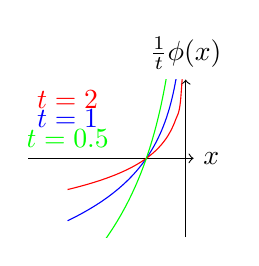
\begin{tikzpicture}
			\draw[->] (-2, 0) -- (0.1, 0) node[right] {$x$};
			\draw[->] (0, -1) -- (0, 1) node[above] {$\frac{1}{t}\phi(x)$};
			
			\clip (-2, -1) rectangle (0.1, 1);
			
			\node[text=red] (rlabel) at (-1.5, 0.75) {$t = 2$};
			\node[text=blue] (blabel) at (-1.5, 0.5) {$t = 1$};
			\node[text=green] (glabel) at (-1.5, 0.25) {$t = 0.5$};
			
			\draw[scale=0.5, domain=-3:-0.01, smooth, variable=\x, blue] plot ({\x}, {-log2(-\x)});
			\draw[scale=0.5, domain=-3:-0.01, smooth, variable=\x, red]  plot ({\x}, {-0.5*log2(-\x)});
			\draw[scale=0.5, domain=-3:-0.01, smooth, variable=\x, green]  plot ({\x}, {-2*log2(-\x)});
		\end{tikzpicture}
	\end{center}

	\textbf{Approximated P-OP}:
	\begin{emphbox}
		$\min\limits_{\bm{x}} f(\bm{x}) + \sum\limits_{i=1}^{l} - \frac{1}{t} \log(-g_i(\bm{x})) \quad \text{s.t.} \bm{A}\bm{x} = \bm{b}$
	\end{emphbox}
	\vspace{0.5em}
	
	\textbf{Central Path}: $\hat{\bm{x}}(t), t > 0$ that satisfy DF
	\vspace{0.3em}
	\begin{center}
		$\bm{0} = t\nabla f(\hat{\bm{x}}(t)) + \nabla\phi(\hat{\bm{x}}(t)) + \bm{A}^\intercal\hat{\bm{v}}$
	\end{center}
	\vspace{0.5em}
	
	\textbf{Duality Gap}:
	\begin{emphbox}
		$f(\hat{\bm{x}}(t)) - p^* \leq \frac{l}{t}$
	\end{emphbox}

\end{sectionbox}

\begin{sectionbox}
	\subsection{KKT Interpretation of P-OP}
	
	\textbf{Primal Feasibility}: \\
	\begin{center}
		$\bm{A}\bm{x} = \bm{b}, \qquad g_i(\bm{x}) < 0$
	\end{center}
	\vspace{0.5em}
	
	\textbf{Dual Feasibility}: \\
	\begin{center}
		$\nabla f(\bm{x}) + \sum\limits_{i=1}^{l} u_i \nabla g_i(\bm{x}) + \bm{A}^\intercal\bm{v} = \bm{0}$ \\
		$\bm{u} \geq \bm{0}$
	\end{center}
	\vspace{0.5em}
	
	\textbf{Complementary Slackness}: \\
	\begin{center}
		$ -u_i g_i(\bm{x}) = \frac{1}{t} $
	\end{center}

	$\implies$ CS is relaxed such that no $g_i$ are active
	
\end{sectionbox}

\begin{sectionbox}
	\subsection{Primal Interior Point Algorithm}
	\vspace{0.5em}
	\textbf{P-OP}: \\
	\begin{center}
		$\min\limits_{\bm{x}} \bm{c}^\intercal\bm{x} - \tau \sum\limits_{j=1}^{n} \log(x_j) \qquad \text{s.t.} \bm{A}\bm{x} = \bm{b}, \bm{x} \geq 0$
	\end{center}
	\vspace{0.5em}
	
	\textbf{PF}:
	\begin{center}
		$\bm{A}\bm{x} = \bm{b}, \qquad \bm{x} \geq \bm{0}$
	\end{center}
	\vspace{0.5em}
	
	\textbf{DF}:
	\begin{center}
		$\bm{c} - \tau \sum\limits_{j=1}^{n} \frac{1}{x_j}e_j - \bm{A}^\intercal \bm{y} = \bm{0} $
	\end{center}

	\textbf{Resulting System}:
	\begin{align}
		\bm{c} - \tau \bm{X}^{-1}\mathbf{1} - \bm{A}^\intercal\bm{y} = & \bm{0} \notag\\
		\bm{A}\bm{x} - \bm{b} = & \bm{0} \qquad \iff \bm{F}(\bm{x}, \bm{y}) = \bm{0}, \bm{x} \geq \bm{0} \notag\\
		\bm{x} \geq & \bm{0} \notag
	\end{align}
	\vspace{0.5em}
	
	\textbf{Newton Step}:
	\begin{center}
		$\begin{bmatrix}
			\Delta \bm{x} \\
			\Delta \bm{y}
		\end{bmatrix} = (\nabla_{\bm{x}, \bm{y}}\bm{F}(\bm{x}, \bm{y}))^{-1}\bm{F}(\bm{x}, \bm{y})$
	\end{center}
	\vspace{0.5em}
	
	\textbf{Newton Update}:
	\begin{center}
		$\begin{bmatrix}
			\bm{x} \\
			\bm{y}
		\end{bmatrix}^{\text{(k+1)}} = \begin{bmatrix}
		\bm{x} \\
		\bm{y}
	\end{bmatrix}^{\text{(k)}} + \alpha \begin{bmatrix}
	\Delta \bm{x} \\
	\Delta \bm{y}
\end{bmatrix}$ \\
		\vspace{0.3em}
		With $\alpha$ such that $\bm{x} \geq \bm{0}$ is not violated!
	\end{center}
	
\end{sectionbox}

\begin{sectionbox}
	\subsection{Primal-Dual Interior Point Algorithm}
	\vspace{0.5em}
	\textbf{P-OP}: \\
	\begin{center}
		$\min\limits_{\bm{x}} \bm{c}^\intercal\bm{x} - \tau \sum\limits_{j=1}^{n} \log(x_j) \qquad \text{s.t.} \bm{A}\bm{x} = \bm{b}, \bm{x} \geq 0$
	\end{center}
	\vspace{0.5em}
	
	\textbf{D-OP}: \\
	\begin{center}
		$\max\limits_{\bm{y}} \bm{b}^\intercal\bm{y} \qquad \text{s.t.} \bm{A}^\intercal\bm{y} + \bm{u} = \bm{0}, \bm{u} \geq 0$
	\end{center}
	\vspace{0.5em}
	
	\textbf{PF}:
	\begin{center}
		$\bm{A}\bm{x} = \bm{b}, \qquad \bm{x} \geq \bm{0}$
	\end{center}
	\vspace{0.5em}
	
	\textbf{DF}:
	\begin{center}
		$\bm{c}^\intercal - \bm{A}^\intercal\bm{y} - \bm{u} = \bm{0} \qquad \text{s.t.} \bm{u} \geq \bm{0} $
	\end{center}
	\vspace{0.5em}

	\textbf{CS}: Is relaxed for better numerical behaviour
	\begin{center}
		$\bm{X}\bm{U}\mathbf{1} = 0 \quad \implies \quad \bm{X}\bm{U}\mathbf{1} = \tau\mathbf{1} \iff \bm{u} = \bm{X}^{-1}\tau\mathbf{1}$
	\end{center}
	\vspace{0.5em}
	
	\textbf{Resulting System}:
	\begin{align}
		\bm{A}^\intercal\bm{y} + \tau \bm{X}^{-1}\mathbf{1} - \bm{c} = & \bm{0} \notag\\
		\bm{A}\bm{x} - \bm{b} = & \bm{0} \qquad \iff \bm{F}(\bm{x}, \bm{y}, \bm{u}) = \bm{0}, \begin{bmatrix}
			\bm{x} \\
			\bm{u}
		\end{bmatrix} \geq \bm{0} \notag\\
		\begin{bmatrix}
			\bm{x} \\
			\bm{u}
		\end{bmatrix} \geq & \bm{0} \notag
	\end{align}
	\vspace{0.5em}
	
	\textbf{Solve for Newton Step}:
	\begin{center}
		$\bm{F}(\bm{x}, \bm{y}, \bm{u}) + \nabla_{\bm{x}, \bm{y}, \bm{u}}\bm{F}(\bm{x}, \bm{y}, \bm{u}) \begin{bmatrix}
			\Delta \bm{x} \\
			\Delta \bm{y} \\
			\Delta \bm{u} \\
		\end{bmatrix} = \bm{0}$
	\end{center}
	\vspace{0.5em}
	
	\textbf{Newton Update}:
	\begin{center}
		$\begin{bmatrix}
			\bm{x} \\
			\bm{y} \\
			\bm{u} \\
		\end{bmatrix}^{\text{(k+1)}} = \begin{bmatrix}
		\bm{x} \\
		\bm{y} \\
		\bm{u} \\
	\end{bmatrix}^{\text{(k)}} + \alpha \begin{bmatrix}
	\Delta \bm{x} \\
	\Delta \bm{y} \\
	\Delta \bm{u} \\
\end{bmatrix}$ \\
		\vspace{0.5em}
		With $\alpha$ such that $\begin{bmatrix}
			\bm{x} \\
			\bm{u} \\
		\end{bmatrix} \geq \bm{0}$ is not violated!
	\end{center}
	
\end{sectionbox}

\pagebreak

\section{Matrix Calculus}

\begin{sectionbox}
	\textbf{Denominator layout convention} \\
	\begin{center}
		$\bm{x}, \bm{a} \in \mathbb{R}^n, \quad \bm{u} \in \mathbb{R}^m \quad \bm{A} \in \mathbb{R}^{m \times n}, \quad \bm{C} \in \mathbb{R}^{n \times n}$
	\end{center}

	\begin{align}
		\frac{\partial \bm{a}^\intercal \bm{x}}{\partial \bm{x}} & = \frac{\partial \bm{x}^\intercal \bm{a}}{\partial \bm{x}} = \bm{a} \\
		\frac{\partial \bm{A} \bm{x}}{\partial \bm{x}} & = \bm{A}^\intercal \\
		\frac{\partial \bm{u}^\intercal\bm{A}\bm{x}}{\partial \bm{x}} & = \bm{A}^\intercal\bm{u}\\
		\frac{\partial \bm{x}^\intercal \bm{C} \bm{x}}{\partial \bm{x}} & = \big( \bm{C} + \bm{C}^\intercal \big)\bm{x} \\
		\frac{\partial}{\partial \bm{x}} \| \bm{x} - \bm{a} \|_2 & = \frac{\bm{x} - \bm{a}}{\| \bm{x} - \bm{a} \|_2} \\
		\frac{\partial}{\partial \bm{x}} \frac{\bm{x} - \bm{a}}{\| \bm{x} - \bm{a} \|_2} & = \frac{\bm{I}}{\| \bm{x} - \bm{a} \|_2} - \frac{(\bm{x} - \bm{a})(\bm{x} - \bm{a})^\intercal}{\| \bm{x} - \bm{a} \|_2^3} \\
		\frac{\partial \| \bm{x} \|_2^2}{\partial \bm{x}} & = \frac{\partial \| \bm{x}^\intercal \bm{x} \|_2}{\partial \bm{x}} = 2 \bm{x}
	\end{align}

\end{sectionbox}


\section{Polyhedral Set Conversions}

\begin{sectionbox}
	\textbf{Primal Standard Form $\implies$ Dual Standard Form}
	\begin{center}
		$\pazocal{S}_p = \{ \bm{x} \in \mathbb{R}^n \mid \bm{A}\bm{x} = \bm{b}, \bm{x} \geq \bm{0} \}$ \\
		\vspace{0.5em}
		$\bm{A}\bm{x} \leq \bm{b}, \quad -\bm{A}\bm{x} \leq -\bm{b}, \quad -\bm{x} \leq \bm{0}$ \\
		\vspace{0.5em}
		$\pazocal{S}_d = \{ \bm{x} \in \mathbb{R}^n \mid \begin{bmatrix}
			\bm{A} \\
			-\bm{A} \\
			-\bm{I} \\
		\end{bmatrix} \bm{x} \leq \begin{bmatrix}
		\bm{b} \\
		-\bm{b} \\
		\bm{0} \\
	\end{bmatrix} \}$
	\end{center}
	\vspace{1em}
	\textbf{Dual Standard Form $\implies$ Primal Standard Form}
	\begin{center}
		$\pazocal{S}_d = \{ \bm{x} \in \mathbb{R}^n \mid \bm{A}\bm{x} \leq \bm{b}\}$ \\
		\vspace{0.5em}
		$\bm{A}\bm{x}^+ - \bm{A}\bm{x}^- + \bm{s} = \bm{b}, \qquad \bm{x}^+, \bm{x}^-, \bm{s} \geq \bm{0}$ \\
		\vspace{0.5em}
		$\pazocal{S}_p =$ \\
		$\big\{ \begin{bmatrix}
			\bm{x}^+ \\
			\bm{x}^- \\
			\bm{s} \\
		\end{bmatrix} \in \mathbb{R}^{2n+m} \mid \begin{bmatrix}
			\bm{A} & -\bm{A} & \bm{I}
			\end{bmatrix} \begin{bmatrix}
			\bm{x}^+ \\
			\bm{x}^- \\
			\bm{s} \\
		\end{bmatrix} = \bm{b}, \begin{bmatrix}
		\bm{x}^+ \\
		\bm{x}^- \\
		\bm{s} \\
	\end{bmatrix} \geq \bm{0} \big\}$
	\end{center}
\end{sectionbox}

\section{Properties of some Sets}

\begin{sectionbox}
	
	The following assumptions are made for the statements below:
	\begin{center}
		$\bm{x} \in \mathbb{R}^n, \quad \bm{y} \in \mathbb{C}^n, \quad \bm{A} \in \mathbb{R}^{m \times n}, \quad \bm{b} \in \mathbb{R}^m $ \\
		$\bm{Q} \in \mathbb{C}^{n \times n}, \quad \bm{P} \in \mathbb{C}^{m \times n}, \quad \bm{p} \in \mathbb{R}^n$ \\
		$\pazocal{X} \subset \mathbb{R}^n $ is closed and convex
	\end{center}
	
	\begin{tablebox}{@{\hspace{5mm}}c@{\extracolsep\fill}c@{\extracolsep\fill}c@{\extracolsep\fill}c@{\extracolsep\fill}c@{\hspace{5mm}}}
		Set & linear & affine & conic & convex \\ \cmrule
		$\{\bm{x} \mid \bm{A}\bm{x} = \bm{b} \}$ & 	& \cmark &  & \cmark \\
		$\{\bm{x} \mid \bm{A}\bm{x} \leq \bm{b} \}$ &  &  &  & \cmark \\
		$\{\bm{x} \mid \bm{A}\bm{x} \leq \bm{0}, \mathbf{1}^\intercal\bm{A}\bm{x} = 0 \}$ & \cmark & \cmark & \cmark & \cmark \\
		$\{\bm{Q} \mid \bm{y}^H \bm{Q} \bm{y} \geq 0, \forall \bm{y} \mathbb{C}^n \}$ &  &  & \cmark & \cmark \\
		$\{\bm{P} \mid \text{tr}(\bm{P}\bm{P}^H) \leq 1 \}$ &  &  &  & \cmark \\
		$\{\bm{P} \mid \det(\bm{P}^{-1}) \neq 0\}$ &  &  & \cmark &  \\
		$\{\bm{p} \mid \bm{p}^\intercal(\bm{x} - \bar{\bm{x}}) \leq 0, \forall \bm{x} \in \pazocal{X} \}$ & & & \cmark & \cmark \\
		$\{ \emptyset \}$ & \cmark & \cmark & \cmark & \cmark \\
		$\{ \bm{x}_0 \}$ & & \cmark & & \cmark \\
		$\{ \bm{x}_0, \bm{x_1} \mid \bm{x}_0 \neq \bm{x_1} \}$ & & & & \\ 
		
	\end{tablebox}
\end{sectionbox}

\section{Properties of a Norm}

\begin{sectionbox}
	\begin{enumerate}
		\item $\| \bm{x} \| \geq 0$, $\| \bm{x} \| = 0 \iff \bm{x} = 0$
		\item $\| \alpha \bm{x} \| = \mid \alpha \mid \| \bm{x} \|$
		\item $\| \bm{x} + \bm{y} \| \leq \| \bm{x} \| + \| \bm{y} \|$
	\end{enumerate}
	\vspace{0.5em}
	\begin{center}
		Every Norm is a convex function!
	\end{center}
\end{sectionbox}

\section{Infeasible OP Example}
\begin{sectionbox}
	P-OP and D-OP are infeasible simultaneously for this example. \\
	\\
	\textbf{P-OP}:
	\begin{center}
		$\inf\limits_{\bm{x} \in \mathbb{R}^n} \bm{c}^\intercal\bm{x} \qquad \text{s.t. } \bm{A}\bm{x} = \bm{b}, \bm{x} \geq \bm{0}$
	\end{center}
	\textbf{D-OP}:
	\begin{center}
		$\sup\limits_{\bm{y} \in \mathbb{R}^m} \bm{b}^\intercal\bm{y} \qquad \text{s.t. } \bm{A}^\intercal\bm{y} \leq \bm{c}$
	\end{center}
	\begin{center}
		$\bm{A} = \begin{bmatrix}
			1 & -1 & -1 \\
			1 & 0 & -1 \\
		\end{bmatrix}, \quad \bm{b} = \begin{bmatrix}
		1 \\
		0 \\
	\end{bmatrix}, \quad \bm{c} < \bm{0}$
	\end{center}

\end{sectionbox}

\section{Deriving IEQs graphically}

\begin{sectionbox}
	
	\textbf{Green Area is feasible area} \\
	\\
	$\alpha$ is slope of line \\
	
	\begin{tabular}{c c}
		
		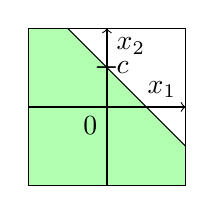
\begin{tikzpicture}[node distance=1cm]
			\coordinate (O) at (0, 0);
			\coordinate (bottomleft) at (-1, -1);
			\coordinate (topright) at (1, 1);
			
			
			\fill[fill=green!30] (bottomleft)--(1, -1)--(1, -0.5)--(-0.5, 1)--(-1, 1);
			\draw[-] (-0.5, 1) -- (1, -0.5);
			\node [] (Cmark) at (0, 0.5) {$\bm{-}$};
			\node [] (Clabel) at (0.2, 0.5) {$c$};
			
			\node[below left] (Olabel) at (O) {$0$};
			
			\draw[->] (-1, 0) -- (1, 0) node [above left] {$x_1$};
			\draw[->] (0, -1) -- (0, 1) node [below right] {$x_2$};
			
			\draw[] (bottomleft) rectangle (topright);
		\end{tikzpicture} &
		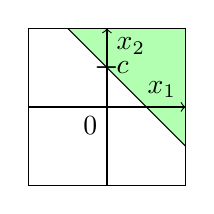
\begin{tikzpicture}[node distance=1cm]
			\coordinate (O) at (0, 0);
			\coordinate (bottomleft) at (-1, -1);
			\coordinate (topright) at (1, 1);
			
			
			\fill[fill=green!30] (topright)--(1, -0.5)--(-0.5, 1);
			\draw[-] (-0.5, 1) -- (1, -0.5);
			\node [] (Cmark) at (0, 0.5) {$\bm{-}$};
			\node [] (Clabel) at (0.2, 0.5) {$c$};
			
			\node[below left] (Olabel) at (O) {$0$};
			
			\draw[->] (-1, 0) -- (1, 0) node [above left] {$x_1$};
			\draw[->] (0, -1) -- (0, 1) node [below right] {$x_2$};
			
			\draw[] (bottomleft) rectangle (topright);
		\end{tikzpicture} \\
		$x_2 \leq \alpha x_1 + c$ & $x_2 \geq \alpha x_1 + c$ \\
		$g(\bm{x}) = x_2 - \alpha x_1 - c \leq 0$ & $g(\bm{x}) = \alpha x_1 + c - x_2 \leq 0 $ \\
		\textit{All $x_2$ below line} & \textit{All $x_2$ above line}
		
	\end{tabular}
	
\end{sectionbox}

\section{Weighted Min Function Contour Lines}

\begin{sectionbox}
	\includegraphics[width=\textwidth]{img/minfunction.pdf}
\end{sectionbox}

\section{Proofs}

\begin{sectionbox}
	\subsection{Proof of the Saddle Point Property}
	
	\begin{align}
		\sup\limits_{x} \inf\limits_{y} f(x, y) \leq & \inf\limits_{y} \sup\limits_{x} f(x, y) \notag \\
		\sup\limits_{x} \inf\limits_{y} f(x, y) = \inf\limits_{y} f(\bar{x}, y) \leq & f(\bar{x}, y) \quad \forall y \text{  (including $\bar{y}$)} \notag\\
		\inf\limits_{y} \sup\limits_{x} f(x, y) = \sup\limits_{x} f(x, \bar{y}) \geq & f(x, \bar{y}) \quad \forall x \text{  (including $\bar{x}$)} \notag
	\end{align}
	
\end{sectionbox}

\begin{sectionbox}
	\subsection{Proof of Farkas Theorem}
	Farkas: Only one system can be true at a time: \\
	\begin{center}
		\begin{enumerate}
			\item $\exists \bm{x} \in \mathbb{R}^n \mid \bm{A}\bm{x} \leq \bm{0}, \bm{c}^\intercal\bm{x} > 0$
			\item $\exists \bm{y} \in \mathbb{R}^m \mid \bm{A}^\intercal\bm{y} = \bm{c}, \bm{y} \leq \bm{0}$
		\end{enumerate}
	\end{center}
	\vspace{0.5em}
	\textbf{If (2) has a solution}: Then there exists $\bm{y} \geq \bm{0}$ that fulfills $\bm{A}^\intercal\bm{y} = \bm{c}$. If \textbf{(1)} would also be true, then $\bm{x}$ has to satisfy $\bm{c}^\intercal\bm{x} = \bm{y}^\intercal\bm{A}\bm{x} > \bm{0}$ which is a contradiction. \\
	\textbf{If (2) has no solution}: Then $\bm{c}$ is \textbf{not} in the cone $\pazocal{A}$ spanned by the columns of $\bm{A}$. Since the cone is closed and convex, there must exist a separating hyperplane that separates all $\bm{x} \in \pazocal{A}$ and $\bm{c}$, which is defined by the normal vector $\bm{p}$. We then have $\bm{p}^\intercal\bm{c} > 0$ and $\bm{p}^\intercal\bm{x} \leq 0$ for all $\bm{x} \in \pazocal{A}$ since $\bm{0} \in \pazocal{A}$. Define $\bm{x} := \bm{A}^\intercal\bm{y}$ yields $\bm{p}^\intercal\bm{A}^\intercal\bm{y} = \bm{y}^\intercal\bm{A}\bm{p} \leq 0$ for $\bm{y} \geq \bm{0}$ which implies $\bm{A}\bm{p} \leq \bm{0}$ with $\bm{c}^\intercal\bm{p} > 0$. This is equal to \textbf{(1)}.
\end{sectionbox}

\begin{sectionbox}
	\subsection{Proof of Gordons Theorem via Farkas Theorem}
	
	\textbf{F1} and \textbf{F2} are System 1 and 2 of Farkas, \textbf{G1} and \textbf{G2} are system 1 and 2 of Gordon. \\
	
	$\textbf{G1: } \bm{A}\bm{x} < \bm{0} \quad \iff \textbf{F1: } \begin{bmatrix}
		\bm{A} & \bm{1}
	\end{bmatrix} \begin{bmatrix}
		\bm{x} \\
		s
	\end{bmatrix} \leq \bm{0} \begin{bmatrix}
			\bm{0}^\intercal & 1
	\end{bmatrix} \begin{bmatrix}
			\bm{x} \\
			s
	\end{bmatrix} > 0$ \\
	$\textbf{F2: } \begin{bmatrix}
		\bm{A}^\intercal \\
		\bm{1}^\intercal
	\end{bmatrix} \bm{y} = \begin{bmatrix}
		\bm{0} \\
		1
\end{bmatrix} \quad \iff \textbf{G2: } \bm{A}^\intercal\bm{y} = \bm{0}, \quad \bm{1}^\intercal\bm{y} = 1, \quad \bm{y} \geq \bm{0}$
	
\end{sectionbox}

\begin{sectionbox}
	\subsection{Proof that the epigraph of a convex function is convex}
	Given two points of the epigraph of a convex function $f$: \\
	\begin{center}
		$[x_1, y_1]^\intercal, [x_2, y_2]^\intercal \in \text{epi}(f)$
	\end{center}
	The definition of convexity yields: \\
	$\lambda y_1 + (1 - \lambda)y_2 \geq \lambda f(x_1) + (1 - \lambda)f(x_2) \geq f(\lambda x_1 + (1-\lambda) x_2)$ \\
	This implies: \\
	\begin{center}
		$\begin{bmatrix}
			\lambda x_1 + (1-\lambda) x_2 \\
			\lambda y_1 + (1-\lambda) y_2
		\end{bmatrix} = \lambda\begin{bmatrix}
			x_1 \\
			y_1
	\end{bmatrix} + (1-\lambda) \begin{bmatrix}
			x_2 \\
			y_2
	\end{bmatrix} \in \text{epi}(f)$
	\end{center}
\end{sectionbox}

\begin{sectionbox}
	\subsection{Proof that the set of subgradients is convex}
	Given two subgradients of $f$ at $\bar{x}$: \\
	\begin{center}
		$f(x) \geq f(\bar{x}) + \xi_1^\intercal(x - \bar{x})$ \\
		$f(x) \geq f(\bar{x}) + \xi_2^\intercal(x - \bar{x})$
	\end{center}
	The definition of convexity yields: \\
	\begin{center}
		$\lambda f(x) + (1-\lambda)f(x) \geq f(\bar{x}) + (\lambda\xi_1^\intercal + (1-\lambda)\xi_2^\intercal)(x - \bar{x})$
	\end{center}
	\textbf{Hence the convex combination of two subgradients is also a subgradient}
\end{sectionbox}



\begin{sectionbox}
	\subsection{Proof of Weak Duality}
	
	\begin{align}
		d^* & = \sup\limits_{v, u \geq 0} \inf\limits_{x \in \pazocal{S}} \{ f(x) + u^\intercal g(x) + v^\intercal h(x) \} \notag\\
		& \leq \sup\limits_{v, u \geq 0} \inf\limits_{x \in \pazocal{X}} \{ f(x) + u^\intercal g(x) + v^\intercal h(x) \} \notag\\
		& \leq \sup\limits_{v, u \geq 0} \{ f(x) + u^\intercal g(x) + v^\intercal h(x) \} \notag\\
		& \leq \sup\limits_{v, u \geq 0} f(x) \notag\\
		& \leq f(x) \notag\\
		& \leq p^* \notag
	\end{align}

	with $\pazocal{S} \subset \pazocal{X}$
	
\end{sectionbox}

\begin{sectionbox}
	\subsection{Proof that the optimizer of a LP is an extremal point}
	From representation theorem, we know that every point $\bm{x}$ in a polyhedron can be represented by the EPs $\bm{x}_i$ and EDs $\bm{d}_j$:
	\begin{center}
		$\bm{x} = \sum\limits_{i=1}^{K} \lambda_i\bm{x}_i + \sum\limits_{j=1}^{L}\mu_j\bm{d}_j, \qquad \sum\limits_{i=1}^{K}\lambda_i = 1$ \\
		$\lambda_i \geq 0, \mu_j \geq 0$ \\
	\end{center}
	A LP can thus be written as:
	\begin{align}
		\min\limits_{\bm{\lambda}, \bm{\mu}} \bm{c}^\intercal \big( \sum\limits_{i=1}^{K} \lambda_i\bm{x}_i + \sum\limits_{j=1}^{L}\mu_j\bm{d}_j \big), \quad \text{s.t. } & \sum\limits_{i=1}^{K}\lambda_i = 1 \notag\\
		& \lambda_i \geq 0, \mu_j \geq 0 \notag
	\end{align}
	where the polyhedral constraint set is enforced by the representation with EPs and EDs. Due to the boundedness requirement for LPs, we have $\bm{c}^\intercal\bm{d}_j \geq 0$ which leads to $\bm{\mu} = \bm{0}$. Therefore, the minimizer is the EP $\bm{x}_i$ with the smallest inner product with $\bm{c}$:
	\begin{center}
		$\bm{x}^* = \argmin\limits_{\bm{x_i}} \{ \bm{c}^\intercal\bm{x}_i \} \qquad \forall i \in \{1, \dots, K\}$
	\end{center}
\end{sectionbox}



% ======================================================================
% End
% ======================================================================
\end{document}
